

\documentclass[twocolumn]{svjour3}       
\journalname{VLDBJ}

%% Font related stuff
%\usepackage{times} 
\usepackage{amsmath} 
\usepackage{amsfonts} 
\usepackage{amssymb} 
%\usepackage{amsthm} 
\usepackage{bold-extra} 
\usepackage[T1]{fontenc} % prettier curly braces in tt mode
\usepackage[scaled]{beramono}
% prettier emptyset
\let\oldemptyset\emptyset
\let\emptyset\varnothing
\DeclareMathOperator{\dist}{dist}

%% Algorithms
\usepackage{listings}
\usepackage[ruled,vlined]{algorithm2e}
\DontPrintSemicolon
\renewcommand{\CommentSty}[1]{\textnormal{#1}}
\SetKwComment{tcp}{$\triangleright$ }{}
\SetVlineSkip{0cm}
\SetAlgoSkip{}


%% others
\usepackage{alltt}
\usepackage{color}
\usepackage{url}
\usepackage[pdftex]{hyperref}
\usepackage{graphicx}
\usepackage{multirow}
\usepackage{blkarray}
\usepackage{balance}
\usepackage{mdframed}

%\usepackage{enumitem}
%\setlist{nolistsep}
%\usepackage{natbib}
%\usepackage[small,compact]{titlesec}
%\titlespacing*{\section}{0pt}{2pt}{1pt}
%\titlespacing*{\subsection}{0pt}{2pt}{1pt}
%\titlespacing*{\subsubsection}{0pt}{2pt}{1pt}
%\titlespacing*{\paragraph}{0pt}{1.75pt}{3pt}
%\usepackage[small,bf,center]{caption}

%% For using smaller font for urls
\makeatletter \def\url@leostyle{\@ifundefined{selectfont}{\def\UrlFont{\sf}}{\def\UrlFont{\scriptsize\ttfamily}}} \makeatother
\urlstyle{leo}

\smartqed  % flush right qed marks
\raggedbottom
%\sloppy 

%% Space savings
%\setlength{\textfloatsep}{0.5\textfloatsep}
%\setlength{\floatsep}{0.5\floatsep}
%\setlength{\intextsep}{0.5\intextsep}
%\setlength{\dbltextfloatsep}{0.5\dbltextfloatsep}
%\setlength{\dblfloatsep}{0.5\dblfloatsep}
%\setlength{\abovecaptionskip}{0.5\abovecaptionskip}
%\setlength{\belowcaptionskip}{0.5\belowcaptionskip}
%\setlength{\footnotesep}{0cm}
%\setlength{\skip\footins}{0.1cm}




\begin{document}
%
% --- Author Metadata here ---
\conferenceinfo{WOODSTOCK}{'97 El Paso, Texas USA}
%\CopyrightYear{2007} % Allows default copyright year (20XX) to be over-ridden - IF NEED BE.
%\crdata{0-12345-67-8/90/01}  % Allows default copyright data (0-89791-88-6/97/05) to be over-ridden - IF NEED BE.
% --- End of Author Metadata ---


\title{Adaptive Disk Storage for Interaction Graphs}


\numberofauthors{2} 
\author{
\alignauthor
Robert Soul\'{e}\\
       \affaddr{University of Lugano}\\
       \email{robert.soule@usi.ch}  
\alignauthor
Bu\u{g}ra Gedik\\
       \affaddr{Bilkent University}\\
       \email{bgedik@cs.bilkent.edu.tr}
}

\maketitle
\begin{abstract}
  TODO
            
\end{abstract}

% A category with the (minimum) three required fields
\category{H.4}{Information Systems Applications}{Miscellaneous}
%A category including the fourth, optional field follows...
\category{D.2.8}{Software Engineering}{Metrics}[complexity measures, performance measures]

\terms{Theory}

\keywords{ACM proceedings, \LaTeX, text tagging}

\section{Introduction}


Graph databases, and \emph{interaction graph} databases in
particular, are a critical component for many of today's most popular
applications.  Graph databases store entities as vertices, relationships as
edges, and have data associated with either vertices or edges, called
\emph{attributes} or \emph{properties}.  Interaction graphs differ from general
graphs in that they are \emph{append-only}, and edges are assigned a
\emph{temporal value}.  Thus, interaction graphs encode the relationships over
time between entities in their structure, making them ideal for use in social
networking, telecommunications, or modeling the world-wide web.

To query an interaction graph, most algorithms traverse the graph structure to
access the relevant attributes.  Frequently, there are correlations among the
attributes accessed by different queries. For example, queries $q_1$ and $q_5$
might access attributes $a_1$ and $a_2$, while queries $q_2$, $q_3$ and $q_4$
access attributes $a_3$ and $a_4$. Because interaction graphs are temporal, the
co-access correlations for the attributes can vary for different
temporal regions.  Moreover, the co-access correlations might be unknown at the
insertion time, but be discovered later, when the workload is known.

It is widely recognized that query workload and disk layout have a significant
impact on database performance~\cite{alagiannis14,grund10,stonebraker05}.  For
table-based, relational databases, this fact has led database designers to
develop alternative approaches for storage layout: row-oriented storage is more
efficient when queries access many attributes from a small number of records,
and column-oriented storage is more efficient when queries access a small number
of attributes from many records~\cite{stonebraker05}.  Unfortunately, although
interaction graph databases, like relational databases, are the target of
diverse query workloads, there is no clear correspondence to a row-oriented or
column-oriented storage layout.

Typically, an interaction graph database is organized as blocks of temporal
neighbor lists.  Attributes can be stored in two ways, either separately (e.g., in a relational
table), or locally with the temporal neighbor lists.  If they are stored
separately, then the graph database cannot take advantage of locality
optimizations performed for block organization.  As discussed in Gedik et
al.~\cite{gedik14}, the database must go back and forth between the disk blocks
to access the edge attributes.  On the other hand, if attributes are stored
locally in the disk blocks containing the graph structure, then there can be
significant overhead due to disk I/O if only a few attributes are needed to
answer a query.

This paper presents an algorithm for adaptively optimizing disk block storage
for interaction graphs. The key idea behind the approach is a novel storage
scheme, called a \emph{rail layout}.  Initially, attributes are stored with
their neighbor lists in large blocks. Over time, the blocks are split into
smaller-blocks that contain the neighbor lists, but only subsets of the
attributes, depending on the query workload. Intuitively, this is almost like
having two or more graph databases for certain time regions, each containing a
different subset of the attributes, but with a link between them in case a query
needs to access both.

\section{Problem Description}

The problem is to determine a partitioning of the disk blocks into sub-blocks
that would minimize query I/O. Of course, partitioning into sub-blocks results
in an increase in storage cost. The storage cost must stay below some
specified limit.

There are two possibilities: \emph{overlapping} and \emph{non-overlapping}
partitioning. In the overlapping case, attributes can be replicated in the
sub-blocks. The non-overlapping case is a true partition.

We start by defining the cost model, which formalizes the query I/O and storage
costs.

\subsection{Cost Model}
Let $Q$ be the query workload, where each query $q\in Q$ accesses a set of
attributes $q.A$ and traverses parts of the graph for the time range
$q.T=[q.t_s,q.t_e]$. We denote the set of all attributes as $A$. Given a block
$B$, we denote its time range as $B.T$, which is the union of the time ranges
of its temporal neighborlists. Let $s(a)$ denote the size of an attribute $a$.
We use $c_n(B)$ to denote the number of temporal neighborlists within block
$B$ and $c_e(B)$ to denote the total number of edges in the temporal
neighborlists within the block. We overload the notation for block size and
use $s(B)$ to denote the size of a block $B$. We have: 
\begin{equation}
s(B) = c_e(B) \cdot \Big(16 + \sum_{a\in B.A} s(a)\Big) + c_n(B) \cdot 12  
\end{equation}
Here, $16$ corresponds to the cost of storing the edge id and the timestamp,
and $12$ corresponds to the cost of storing the head vertex ($8$ bytes) plus
the number of entries ($4$ bytes) for a temporal neighborlist. 

Our goal is to create a potentially overlapping partitioning of a block,
denoted by $\mathcal{P}(B)$. We call the partitions \emph{sub-blocks}. We have
$\bigcup_{B'\in \mathcal{P}(B)} B'.A = A$. We aim to find the function
$\mathcal{P}$ that minimizes the query I/O over $B$, while keeping the
relative storage overhead beyond a limit, say $1+\alpha$ times the original.
If we represent the query I/O as $L(\mathcal{P}, B)$ and the relative storage
overhead as $H(\mathcal{P}, B)$, our goal is to find:
\begin{equation}
\mathcal{P} \leftarrow \mbox{argmin}_{\{\mathcal{P}: H(\mathcal{P}(B)) < \alpha\}} L(\mathcal{P},B)
\end{equation}

The storage overhead can be formalized as follows for the non-overlapping case:
\begin{equation}
H(\mathcal{P}, B) = (|\mathcal{P}(B)|-1)\cdot\Big(1-\frac{c_e(B)\cdot \sum_{a\in A} s(a)}{s(B)}\Big) 
\end{equation}

For the general case (including overlapping), we can formulate the storage
overhead as follows:
\begin{equation}
H(\mathcal{P}, B) = \frac{\sum_{B'\in \mathcal{P}(B)} s(B')}{s(B)} - 1 
\end{equation}

%TODO: note about why we have two different cases

\subsubsection{Query I/O}

Let $m$ be a function that maps a query $q$ to the set of sub-blocks that are
accessed to satisfy it for a relevant block $B$ under a given partitioning
$\mathcal{P}$. For the case of non-overlapping attributes, we have:
\begin{equation}
m(\mathcal{P}, B, q) = \{B': B'\in \mathcal{P}(B) \wedge q.A \cap B'.A \ne \emptyset\}  
\end{equation}

For the case of overlapping attributes, we use a simple heuristic to define the
set of sub-blocks to be used for answering the query.
Algorithm~\ref{alg:greedyM} captures it. The idea is to select sub-blocks that
bring the highest relative marginal gain, which is defined as the size of
attribute data that contributes to the query result, relative to the sub-block
size. While computing the marginal gain, attributes that are covered by
sub-blocks that are already selected are not considered.
%
\begin{algorithm}[ht]
\scriptsize
\caption{m-overlapping($\mathcal{P}, B, q$)}
\label{alg:greedyM}
\KwData{$\mathcal{P}$: partitioning function, $B$: block, $q$: query}
$S\leftarrow \emptyset; R\leftarrow \emptyset$ \tcp*{Selected attributes; Resulting sub-blocks}
\While(\tcp*[f]{While unselected attributes remain}){$S \subset q.A$}{
  $B' \leftarrow \mbox{argmax}_{B'\in\mathcal{P}(B)\setminus R} \sum_{a\in B'.A \cap q.A \setminus S} \frac{c_e(B') \cdot s(a)}{s(B')}$
  $S \leftarrow S \cup B'.A$\tcp*{Extend the selected attributes}
  $R\leftarrow R \cup B'$\tcp*{Extend the selected sub-blocks}
}
\Return R \tcp*{Final set of sub-blocks covering the query attributes}
\end{algorithm} 
%
The query I/O cost for a block is then given by:
\begin{equation}
L(\mathcal{P}, B) = \sum_{q\in Q} w(q)\cdot\mathbf{1}(q.T \cap B.T \neq \emptyset) \cdot \sum_{B'\in m(\mathcal{P}, B, q)} \!\!s(B')
\end{equation}

Here, $w(q)$ represents the query weight.

%\paragraph{\textbf{Other useful equations}}
%\noindent The following are unused, but may be needed for the partitioning
%algorithm.
%
%Let $f: \mathbb{R}\times A \rightarrow \mathbb{N}$ be a function that maps a
%attribute-timestamp pair $(a, t)$ to the frequency of queries that access
%attribute $a$ for time $t$. More formally:
%\begin{equation}
%f(a,t) = \sum_{q\in Q} \textbf{1}(a\in q.A \wedge t\in q.T)
%\end{equation}
%
%Let $T$ represent a time range $[T.s, T.e]$. We denote the frequency of
%attribute access for the time interval $T$ for attribute $a$ as follows:
%\begin{equation}
%f(a, T) = \int_{T.s}^{T.e} f(a, t)\cdot dt =  \sum_{q\in Q} |q.T \cap T| 
%\end{equation}


\section{Partitioning}
This section is still a work-in-progress. We are trying to find the algorithms.

\subsection{Non-Overlapping Attributes}

\paragraph*{Problem.$\,$} \emph{Find a true partitioning of attributes that
minimizes the query I/O and bounds the storage cost by some upper limit.}

\subsubsection{Integer Linear Program Formulation}\label{subsubsec:nov-ilp}
We present an ILP formuation of the problem. For this purpose, we define a 
number of binary ($0$ or $1$) variables: 
\begin{itemize}
\item $x_{a,p}$: $1$ if attribute $a$ is in partition $p$, $0$ otherwise.
\item $y_{p,q}$: $1$ if partition $p$ is used by query $q$, $0$ otherwise.
\item $z_{a,p,q}$: $1$ if partition $p$ is used by query $q$ and attribute $a$
is in partition $p$, $0$ otherwise.
\item $u_{p}$: $1$ if partition $p$ is assigned at least $1$ attribute, $0$ otherwise.
\end{itemize}

Each of these variables serve a purpose:
\begin{itemize}
\item $x$s define the attribute-to-partition assignment.
\item $y$s help formulate the query I/O contribution
of partitions, excluding their assigned attributes.
\item $z$s help formulate the query I/O contribution
of partitions, only considering their assigned attributes.
\item $u$s help formulate the storage overhead requirement.
\end{itemize}

We also define a helper notation for representing whether a variable is
accessed by a query or not: $q(a)\equiv \mathbf{1}(a \in q.A)$, where
$\mathbf{1}$ is the indicator function. We assume that there are a maximum of
$k$ partitions. $k$ can be taken as $|A|$, as there cannot be more partitions
than there are attributes.

We are now ready to state the ILP formulation. We start with the objective
function, that is the total query I/O:
\begin{eqnarray}
\sum_{q\in Q} w(q) \cdot \Big(\sum_{p=1}^{k} \!\!&&\!\! (16\cdot c_e(B) + 12\cdot c_n(B))\cdot
y_{p,q}\nonumber\\ 
&+& \sum_{a\in A} s(a)\cdot c_e(B)\cdot z_{a,p,q}\Big)\label{eq:no-obj}
\end{eqnarray}

In Eq.~\ref{eq:no-obj}, we simply sum for each query and each partition, and
add the I/O cost of reading in the structural information found in a
sub-block, if the partition is used by the query. We then sum over each
attribute as well, and add the I/O cost of reading in the attributes. Note
that $z_{a,p,q}$ could have been  replaced with $x_{a,p}\cdot y_{p,q}$, but
that would make the objective function non-linear. 

We are now ready to state our constraints. Our first constraint is that, each
attribute must be assigned to a single partition. Formally:
\begin{eqnarray}
\forall_{a\in A}, \sum_{p=1}^{k} x_{a,p} = 1
\end{eqnarray}

Our second constraint is that, if a query $q$ contains an attribute $a$
assigned to a partition $p$, then partition $p$ is used by the query, i.e.,
$y_{p,q}=1$. In essence, we want to state: $\forall_{\{p,q\}\in [1..k]\times
Q}, y_{p,q} = \mathbf{1}(\sum_{a\in A} q(a)\cdot x_{a,p}>0)$. 

In order to formulate this constraint, we use the following ILP  construction:
Assume we have two variables, $\beta_1$ and $\beta_2$, where $\beta_2\in[0,1]$
and $\beta_1\geq 0$. We want to implement the following constraint: $\beta_2 =
\mathbf{1}(\beta_1 > 0)$. This could be expressed as a linear constraint as
follows, where $K$ is a large constant guaranteed to be larger than $\beta_1$
for practical purposes:
\begin{eqnarray}
&& \beta_1 - \beta_2 \geq 0\nonumber\\
&& K\cdot\beta_2 - \beta_1 \geq 0\label{eq:beta-ilp}
\end{eqnarray}

We now apply this construction to our second constraint, where
$\beta_1=\sum_{a\in A} q(a)\cdot x_{a,p}$ and $\beta_2=y_{p,q}$. This results
in the following linear constraints:
\begin{eqnarray}
\forall_{\{p,q\}\in [1..k]\times Q}, 
    &&  \sum_{a\in A} q(a)\cdot x_{a,p} - y_{p,q} \geq 0 \nonumber\\
\forall_{\{p,q\}\in [1..k]\times Q}, 
    &&  K\cdot y_{p,q} - \sum_{a\in A} q(a)\cdot x_{a,p}  \geq 0 
\end{eqnarray}

Our third constraint is that, if an attribute $a$ is assigned to a partition
$p$, and partition $p$ is used by a query $q$, then the corresponding $z$
variable must be set to $1$. That is, we want: $\forall_{\{a,p,q\}\in A\times
[1..k]\times Q}, z_{a,p,q}=\mathbf{1}(x_{a,p} = y_{p,q} = 1)$. We express this
as a linear  constraint, as follows:
\begin{eqnarray}
\forall_{\{a,p,q\}\in A\times [1..k]\times Q},
    && z_{a,p,q} - (x_{a,p} + y_{p,q}) \geq -1\label{eq:no-z}
\end{eqnarray}

In Eq.~\ref{eq:no-z}, when the $x$ and $y$ variables are both $1$, the  $z$
variable is simply forced to be $1$. Otherwise, the $z$ variable can be either
$0$ or $1$, but since the $z$ variables appear in the objective fucntion as
positive terms, the solver will set them to $0$, which is what we want. 

Our fourth constraint is that, if a partition is non-empty, then its
corresponding $u$ variable must be set to $0$. In other words,  we want
$\forall_{p\in[1..k]}, u_p = \mathbf{1}(\sum_{a\in A} x_{a,p}>0)$. This is
expressed as linear constraints, as follows:
\begin{eqnarray}
\forall_{p\in[1..k]},
    && \sum_{a\in A} x_{a,p} - u_p \geq 0 \nonumber\\
\forall_{p\in[1..k]},
    && K\cdot u_p - \sum_{a\in A} x_{a,p} \geq 0 \label{eq:no-u}
\end{eqnarray}

Eq.~\ref{eq:no-u} uses the same construction as the second constraint, where
$\beta_1=\sum_{a\in A} x_{a,p}$ and $\beta_2=u_p$.

Our fifth, and the last, constraint deals with the storage overhead. We want to
 make sure that the storage overhead does not go over $\alpha$. The storage
overhead depends on the number of partitions used. That means that the only 
ILP variables it depends on is the $u$s. In particular, the number of
partitions used is given by $\sum_{p=1}^{k} u_p$. This results in the
following linear constraint:
\begin{equation}
\sum_{p=1}^{k} u_p \leq 1 + \frac{\alpha}
  {1-\frac{c_e(B)\cdot \sum_{a\in A} s(a)}{s(B)}}
\end{equation}

\begin{figure}[!t]
\begin{mdframed}
\begin{eqnarray}
\text{minimize}  
    \sum_{q\in Q} w(q)\cdot \Big(\sum_{p=1}^{k} \!\!&&\!\! (16\cdot c_e(B) + 12\cdot c_n(B))\cdot y_{p,q}\nonumber\\
    &+& \sum_{a\in A} s(a)\cdot c_e(B)\cdot z_{a,p,q} \Big) \nonumber\\
\text{subject to}&&\nonumber\\
\forall_{a\in A}, 
    && \sum_{p=1}^{k} x_{a,p} = 1\nonumber\\
\forall_{\{p,q\}\in [1..k]\times Q}, 
    &&  \sum_{a\in A} q(a)\cdot x_{a,p} - y_{p,q} \geq 0 \nonumber\\
\forall_{\{p,q\}\in [1..k]\times Q}, 
    &&  K\cdot y_{p,q} - \sum_{a\in A} q(a)\cdot x_{a,p}  \geq 0 \nonumber\\
\forall_{\{a,p,q\}\in A\times [1..k]\times Q},
    && z_{a,p,q} - (x_{a,p} + y_{p,q}) \geq -1\nonumber\\
\forall_{p\in[1..k]},
    && \sum_{a\in A} x_{a,p} - u_p \geq 0 \nonumber\\
\forall_{p\in[1..k]},
    && K\cdot u_p - \sum_{a\in A} x_{a,p} \geq 0 \nonumber\\    
&& \sum_{p=1}^{k} u_p \leq 1 + \frac{\alpha}
  {1-\frac{c_e(B)\cdot \sum_{a\in A} s(a)}{s(B)}} \nonumber
\end{eqnarray}
\end{mdframed}
\caption{ILP formulation for the non-overlapping partitioning}
\label{fig:nov-ilp}
\end{figure}

The final ILP formulation for the non-overlapping partitioning is given in
Figure~\ref{fig:nov-ilp}.

\subsubsection{Heuristic Solution}

\paragraph*{Approach.$\,$}
TODO

\begin{algorithm}[ht]
\scriptsize
\caption{Algorithm for partitioning blocks into sub-blocks with non-overlapping attributes.}
\label{alg:non-overlappingP}
\KwData{$B$: block, $Q$: set of queries}
$c^*\leftarrow \infty$ \tcp*{Lowest cost over all \# of partitions}
\For(\tcp*[f]{For each possible \# of partitions}){$k=1$ to $|A|$}{
   $R[i]\leftarrow \emptyset, \forall i\in [1..k]$ \tcp*{Initialize partitions}
   \For(\tcp*[f]{For each attribute}){$a \in A$\textnormal{, in decr.\/ order of }$f(a)$}{
      $c\leftarrow \infty$ \tcp*{Lowest cost over all assignments}  
      $j\leftarrow -1$ \tcp*{Best partition assignment}
      \For(\tcp*[f]{For each partition assignment}){$i\in [1..k]$} {
         $R[i]\leftarrow R[i] \cup \{a\}$\tcp*{Assign attribute}
         \If(\tcp*[f]{If query cost is lower}){$L(R, B, Q)<c$}{
            $c\leftarrow L(R, B, Q)$\tcp*{Update the lowest cost}
            $j\leftarrow i$\tcp*{Update the best partition}
         }
         $R[i]\leftarrow R[i] \setminus \{a\}$\tcp*{Un-assign attribute}
      }
      $R[j]\leftarrow R[j] \cup \{a\}$\tcp*{Assign to best partition}
   }
   \lIf(\tcp*[f]{If solution infeasible}){$H(R, B, Q)>\alpha$}{\textbf{break}}
   \If(\tcp*[f]{If solution has lower cost}){$L(R, B, Q)<c^*$}{
     $c^* \leftarrow L(R, B, Q)$\tcp*{Update the lowest cost}
     $\mathcal{P}(B)\leftarrow R$\tcp*{Update the best partitioning}
   } 
}
\Return $\mathcal{P}(B)$ \tcp*{Final set of sub-blocks}
\end{algorithm} 

\clearpage
\newpage
\subsection{Overlapping Attributes}

\paragraph*{Problem.$\,$} \emph{Find an overlapping partitioning of attributes
that minimizes the query I/O and bounds the storage cost by some upper
limit.}

\subsubsection{Integer Linear Program Formulation}
We present an ILP formuation of the problem, as we did for the case of
non-overlapping partitions in Section~\ref{subsubsec:nov-ilp}. We use the same
set of variables and the same objective function. However, the formulation of
the constraints differ. 

Our first constraint is that, each attribute must be assigned to at leat one
partition. Formally:
\begin{eqnarray}
\forall_{a\in A}, \sum_{p=1}^{k} x_{a,p} \geq 1
\end{eqnarray}

As our second constraint, we require that for each attribute used by a query,
there needs to be a partition that is used by that query and that contains the
attribute in question. Formally:
\begin{eqnarray}
\forall_{\{a,q\}\in A\times Q}, \sum_{p=1}^{k} z_{a,p,q} \geq q(a) 
\end{eqnarray}

\begin{sloppypar}
As our third constraint, we require that if a query is using an attribute from
a partition, then that partition must contain the attribute. I.e., we need
to link the $z$ variables with the $x$ variables as
$\forall_{\{a,p,q\}\in A\times [1..k]\times Q}, (z_{a,p,q} = 1) \implies 
(x_{a,p} = 1)$. This can be state as linear constraints:
\begin{eqnarray}
\forall_{\{a,p,q\}\in A\times [1..k]\times Q}, x_{a,p} - z_{a,p,q} \geq 0 
\end{eqnarray}
\end{sloppypar}

As our fourth constraint, we require that if a query is using at least one
attribute from a partition, then that partition must be used by the query.
I.e., we need to link the $z$ variables with the $y$ variables as
$\forall_{\{p,q\}\in [1..k]\times Q}, y_{p,q} = \mathbf{1}(\sum_{a\in A}
z_{a,p,q}>0)$. As before, we use the ILP construction from
Eq.~\ref{eq:beta-ilp} for this, where $\beta_2=y_{p,q}$ and $\beta_1 =
\sum_{a\in A} z_{a,p,q}$. We get:
\begin{eqnarray}
\forall_{\{p,q\}\in [1..k]\times Q}, 
    &&  \sum_{a\in A} z_{a,p,q} - y_{p,q} \geq 0 \nonumber\\
\forall_{\{p,q\}\in [1..k]\times Q}, 
    &&  K\cdot y_{p,q} - \sum_{a\in A} z_{a,p,q} \geq 0 
\end{eqnarray}

Our fifth constraint is that, if an attribute $a$ is assigned to a partition
$p$, and partition $p$ is used by a query $q$, then the corresponding $z$
variable must be set to $1$. This is same as the formulation for the
non-overlapping case from Eq.~\ref{eq:no-z}.

Our sixth constraint is that, if a partition is non-empty, then its
corresponding $u$ variable must be set to $0$. Again, this is same as the
formulation for the non-overlapping case from Eq.~\ref{eq:no-u}.

Our seventh, and the last, constraint deals with the storage overhead. However,
the storage overhead formulation for the overlapping case is different from 
the one for the non-overlapping. This is because the overhead does not merely
depend on the number of partitions, as attributes might have to be loaded
multiple times from different partitions. As a result, we express the overhead
using base variables as in the objective function. Formally:
\begin{eqnarray}
\sum_{p=1}^{k} \Big((16\cdot c_e(B) &+& 12 \cdot c_n(B)) \cdot u_p  \nonumber \\ 
+ \sum_{a\in A} s(a) \!\!&\cdot&\!\! c_n(B)\cdot x_{a,p} \Big) \leq s(B)\cdot (1+\alpha)
\end{eqnarray}

\begin{figure}[!t]
\begin{mdframed}
\begin{eqnarray}
\text{minimize}  
    \sum_{q\in Q} w(q)\cdot \Big(\sum_{p=1}^{k} \!\!&&\!\! (16\cdot c_e(B) + 12\cdot c_n(B))\cdot y_{p,q}\nonumber\\
    &+& \sum_{a\in A} s(a)\cdot c_e(B)\cdot z_{a,p,q} \Big) \nonumber\\
\text{subject to}&&\nonumber\\
\forall_{a\in A}, 
    && \sum_{p=1}^{k} x_{a,p} \geq 1\nonumber\\
\forall_{\{a,q\}\in A\times Q},
    &&  \sum_{p=1}^{k} z_{a,p,q} \geq q(a) \nonumber\\
\forall_{\{a,p,q\}\in A\times [1..k]\times Q}, 
    && x_{a,p} - z_{a,p,q} \geq 0 \nonumber\\
\forall_{\{p,q\}\in [1..k]\times Q}, 
    &&  \sum_{a\in A} z_{a,p,q} - y_{p,q} \geq 0 \nonumber\\
\forall_{\{p,q\}\in [1..k]\times Q}, 
    &&  K\cdot y_{p,q} - \sum_{a\in A} z_{a,p,q}  \geq 0 \nonumber\\
\forall_{\{a,p,q\}\in A\times [1..k]\times Q}, 
    && z_{a,p,q} - (x_{a,p} + y_{p,q}) \geq -1 \nonumber\\
\forall_{p\in[1..k]},
    && \sum_{a\in A} x_{a,p} - u_p \geq 0 \nonumber\\
\forall_{p\in[1..k]},
    && K\cdot u_p - \sum_{a\in A} x_{a,p} \geq 0 \nonumber\\    
\sum_{p=1}^{k} \Big((16\cdot c_e(B) &+& 12 \cdot c_n(B)) \cdot u_p  \nonumber \\ 
+ \sum_{a\in A} s(a) \!\!&\cdot&\!\! c_n(B)\cdot x_{a,p}  \Big)\leq s(B)\cdot (1+\alpha)\nonumber
\end{eqnarray}
\end{mdframed}
\caption{ILP formulation for the overlapping partitioning}
\label{fig:ov-ilp}
\end{figure}

The final ILP formulation for the overlapping partitioning is given in
Figure~\ref{fig:ov-ilp}.

\subsubsection{Heuristic Solution}

\paragraph*{Approach.$\,$} We start the algorithm with a   partitioning based
on what queries we have seen. Every query gets its own sub-block. This is the
``ideal'' partitioning, because the I/O cost would be minimized for every
query that we would have seen. The algorithm iteratively combines the two
partitions that are closest together.  After each combination of partitions,
the algorithm calculate the storage overhead for the partitioning. The
algorithm stops when the  storage cost is below some specified threshold.  The
result is the block partitioning.

\begin{algorithm}[ht]
\scriptsize
\caption{Algorithm for partitioning blocks into sub-blocks with overlapping attributes.}
\label{alg:overlappingP}
\KwData{$B$: block, $Q$: set of queries}
$\mathcal{P}(B) \leftarrow \{q.A: q\in Q\}$ \tcp*{Each query gets its own sub-block}
\While(\tcp*[f]{Until storage overhead is below $\alpha$}){$H(\mathcal{P},B) > \alpha$}{
  $c^{*}\gets \infty $ \tcp*{Lowest cost over all sub-block pairs}
  $(b_x,b_y)\gets (\emptyset,\emptyset)$ \tcp*{Sub-block pair with the lowest cost}
  \For(\tcp*[f]{For each pair of blocks}){$\{b_i,b_j\}\in\mathcal{P}(B)$}{
    $\mathcal{P'}(B) \leftarrow \mathcal{P}(B) \setminus \{b_i, b_j\} \cup \{b_i \cup b_j\}$\\
    $c\gets \frac{L(\mathcal{P}',B,Q)-L(\mathcal{P},B,Q)}{H(\mathcal{P},B)-H(\mathcal{P}',B)}$\tcp*{Cost of merge}
    \If(\tcp*[f]{Cost is lower}){$c<c^{*}$}{
        $c^{*}\gets c$\tcp*{Update the lowest cost}
        $(b_x,b_y)\gets (b_i,b_j)$\tcp*{Update the best pair}
    }
  }
  $\mathcal{P}(B) \leftarrow \mathcal{P}(B) \setminus \{b_x, b_y\} \cup \{b_x \cup b_y\}$ \\
}
\Return $ \mathcal{P}(B)$  \tcp*{Final set of sub-blocks}
\end{algorithm} 



\section{Evaluation}


 \begin{figure*}[ht!]
 \centerline{\begin{tabular}{c@{ }c@{ }c}
 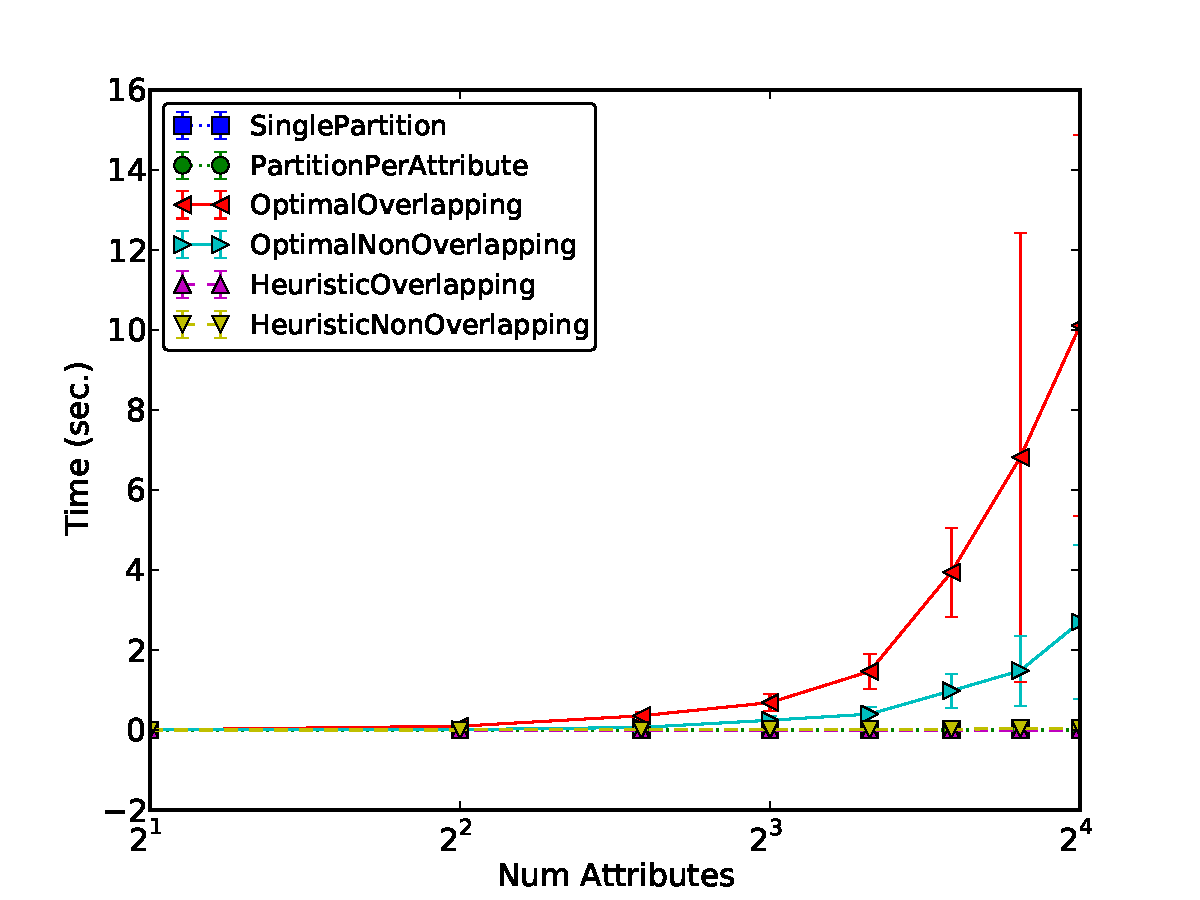
\includegraphics[width=0.33\textwidth]{figures/RunningTimeVsNumAttributes.pdf} &
 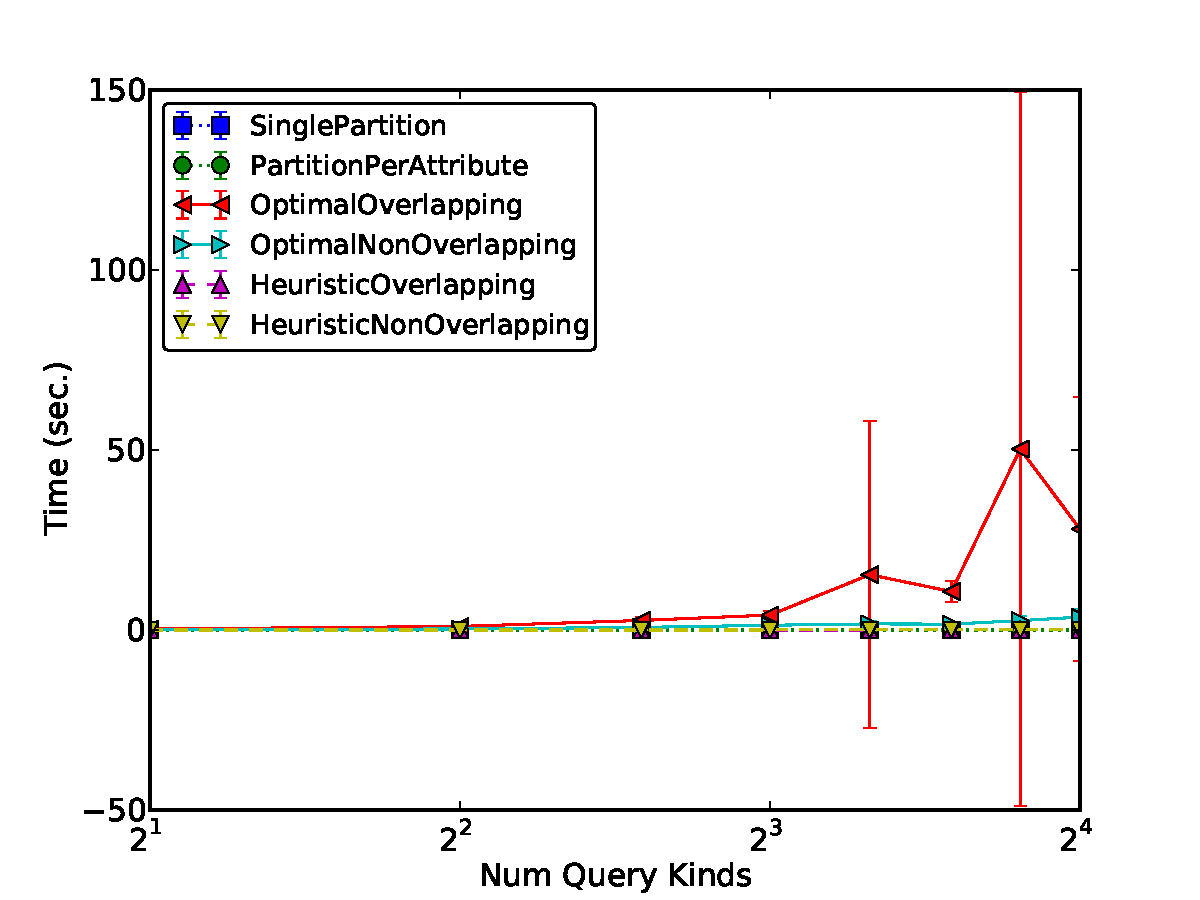
\includegraphics[width=0.33\textwidth]{figures/RunningTimeVsNumQueryKinds.pdf} &
 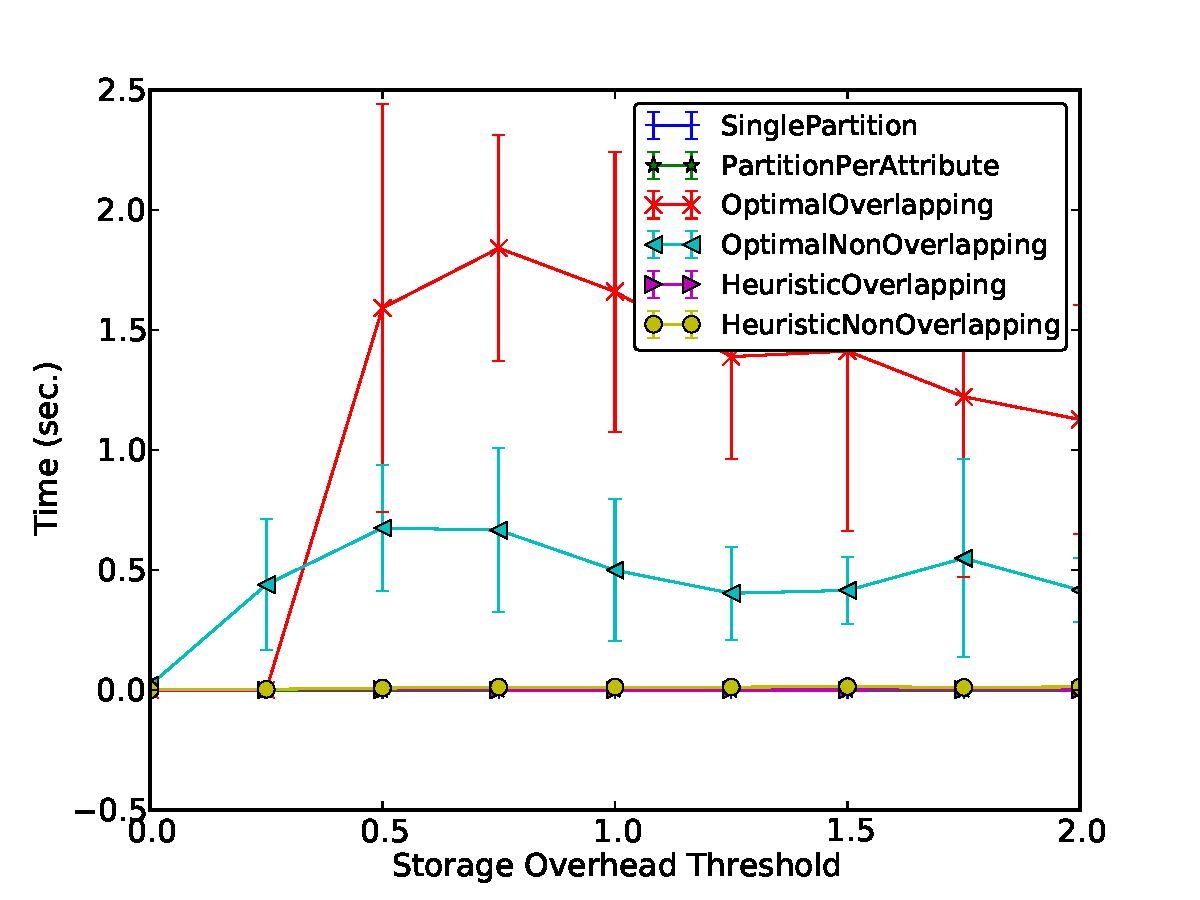
\includegraphics[width=0.33\textwidth]{figures/RunningTimeVsStorageOverheadThreshold.pdf}\\
 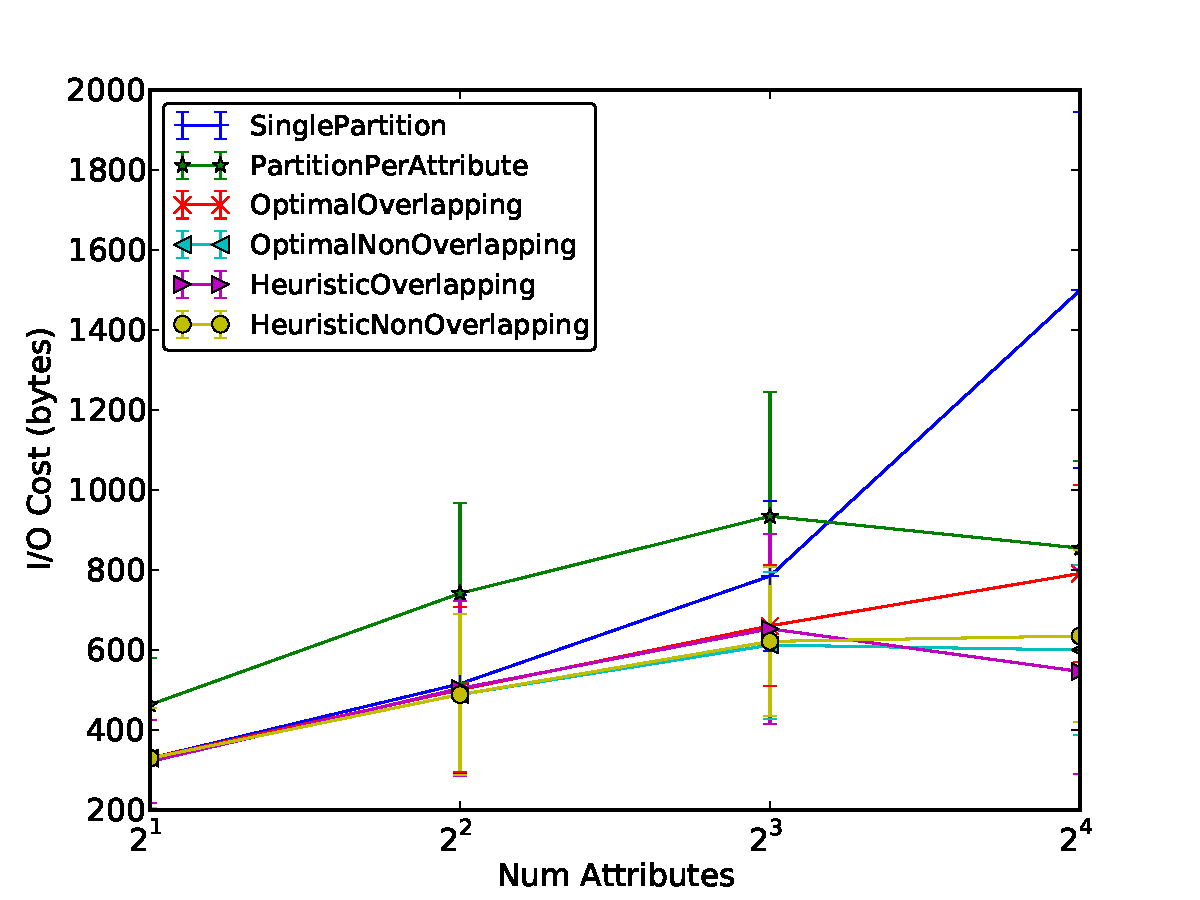
\includegraphics[width=0.33\textwidth]{figures/QueryIOVsNumAttributes.pdf} &
 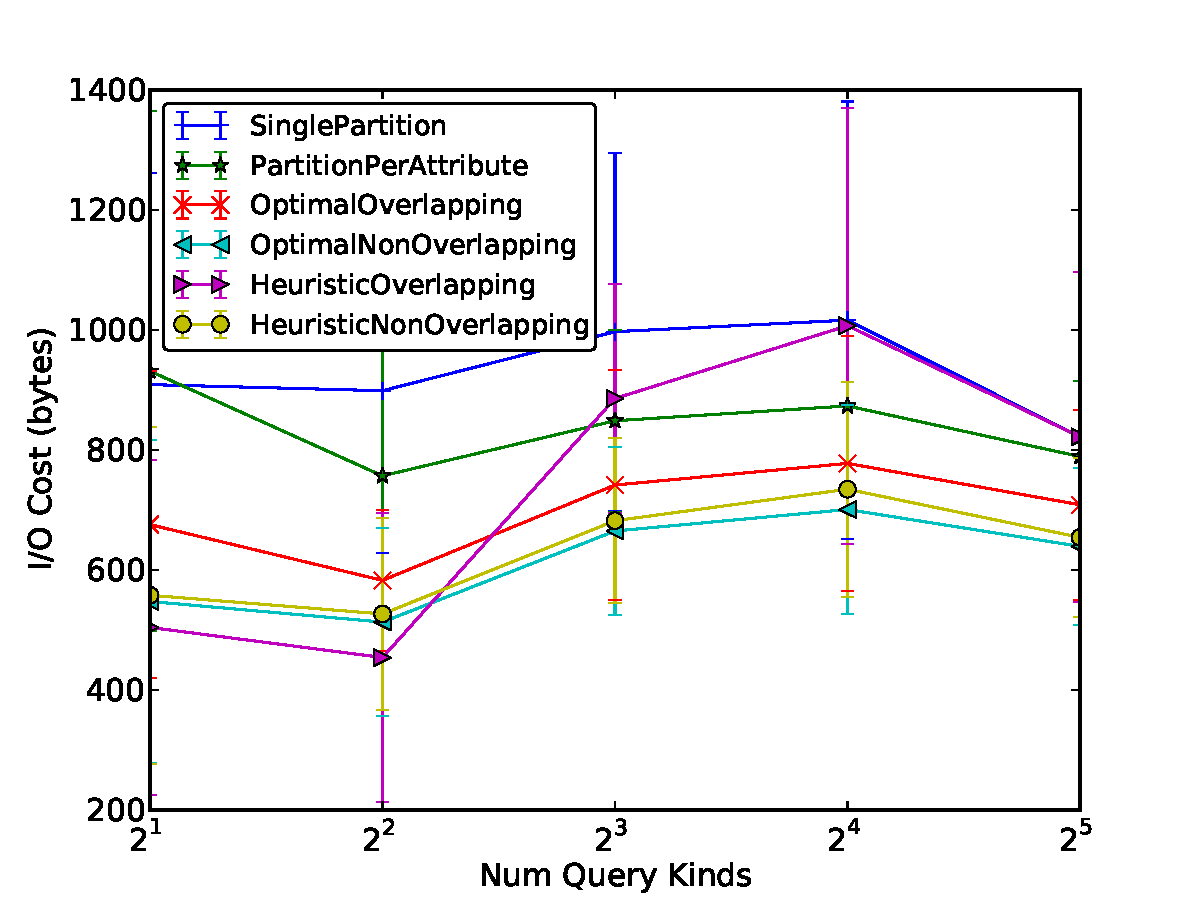
\includegraphics[width=0.33\textwidth]{figures/QueryIOVsNumQueryKinds.pdf} &
 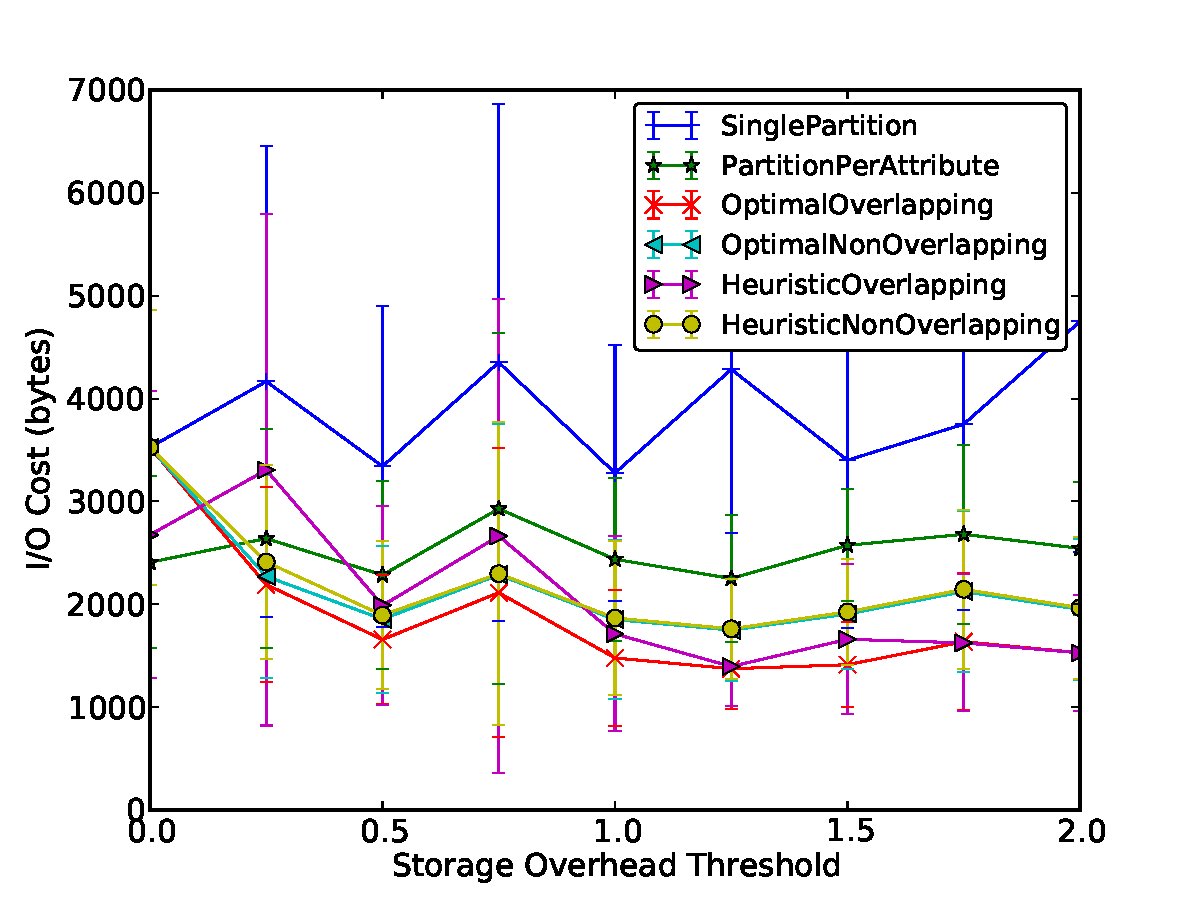
\includegraphics[width=0.33\textwidth]{figures/QueryIOVsStorageOverheadThreshold.pdf}\\
 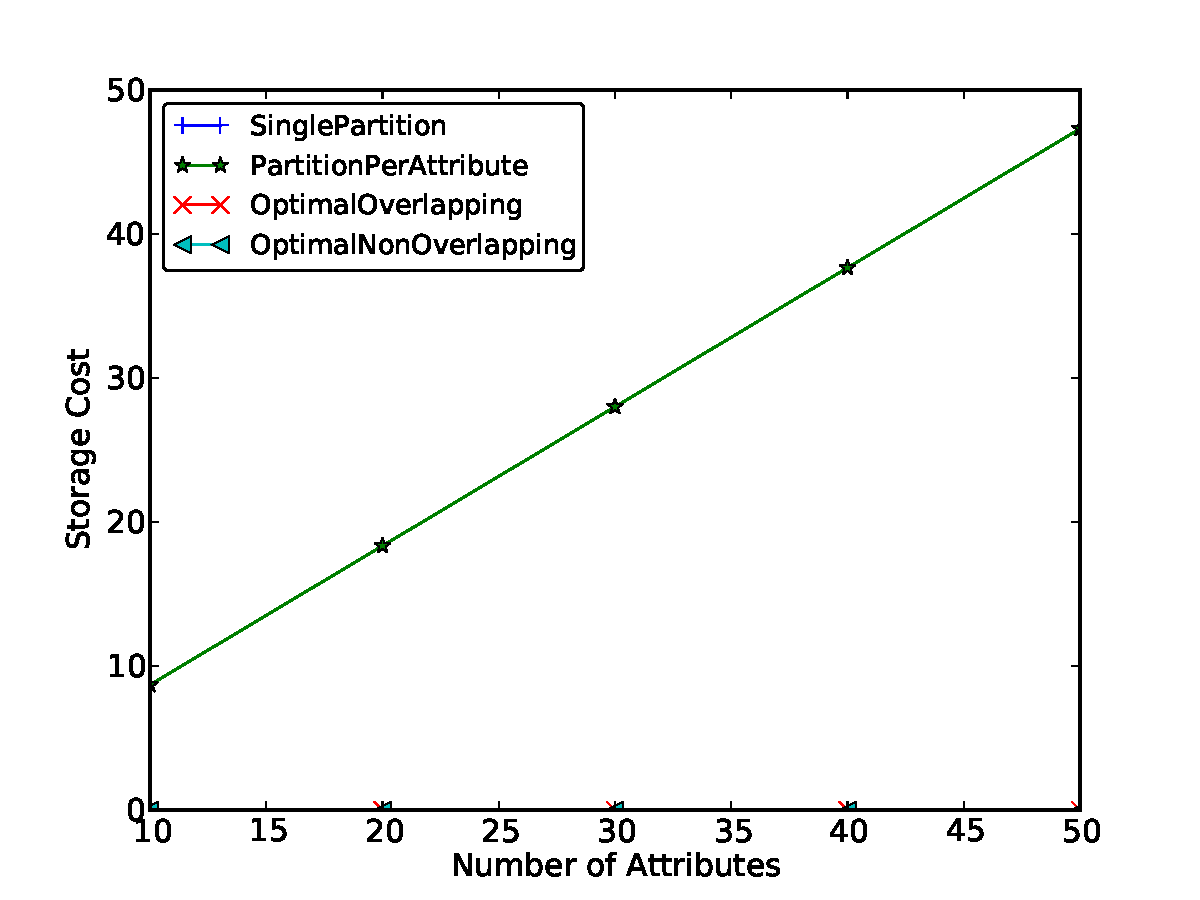
\includegraphics[width=0.33\textwidth]{figures/StorageOverheadVsNumAttributes.pdf} &
 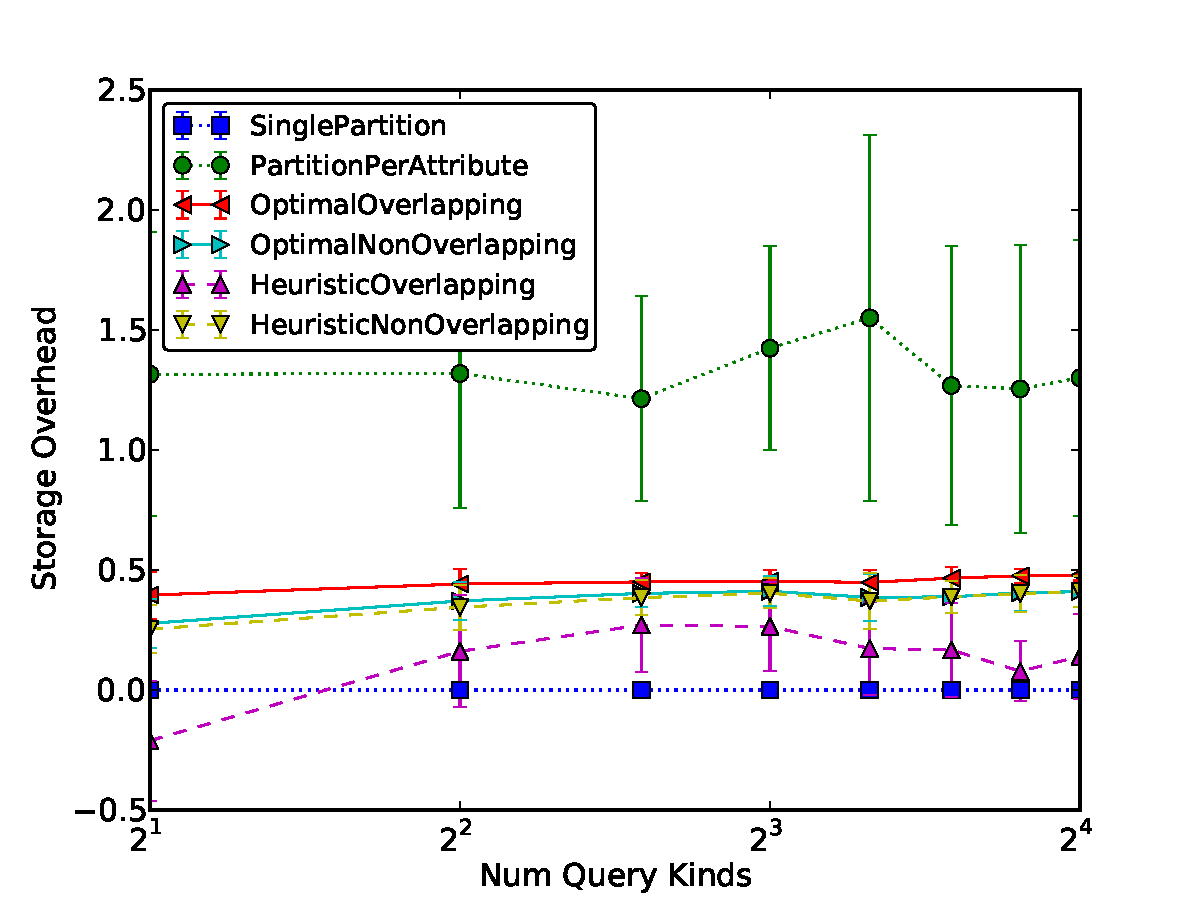
\includegraphics[width=0.33\textwidth]{figures/StorageOverheadVsNumQueryKinds.pdf} &
 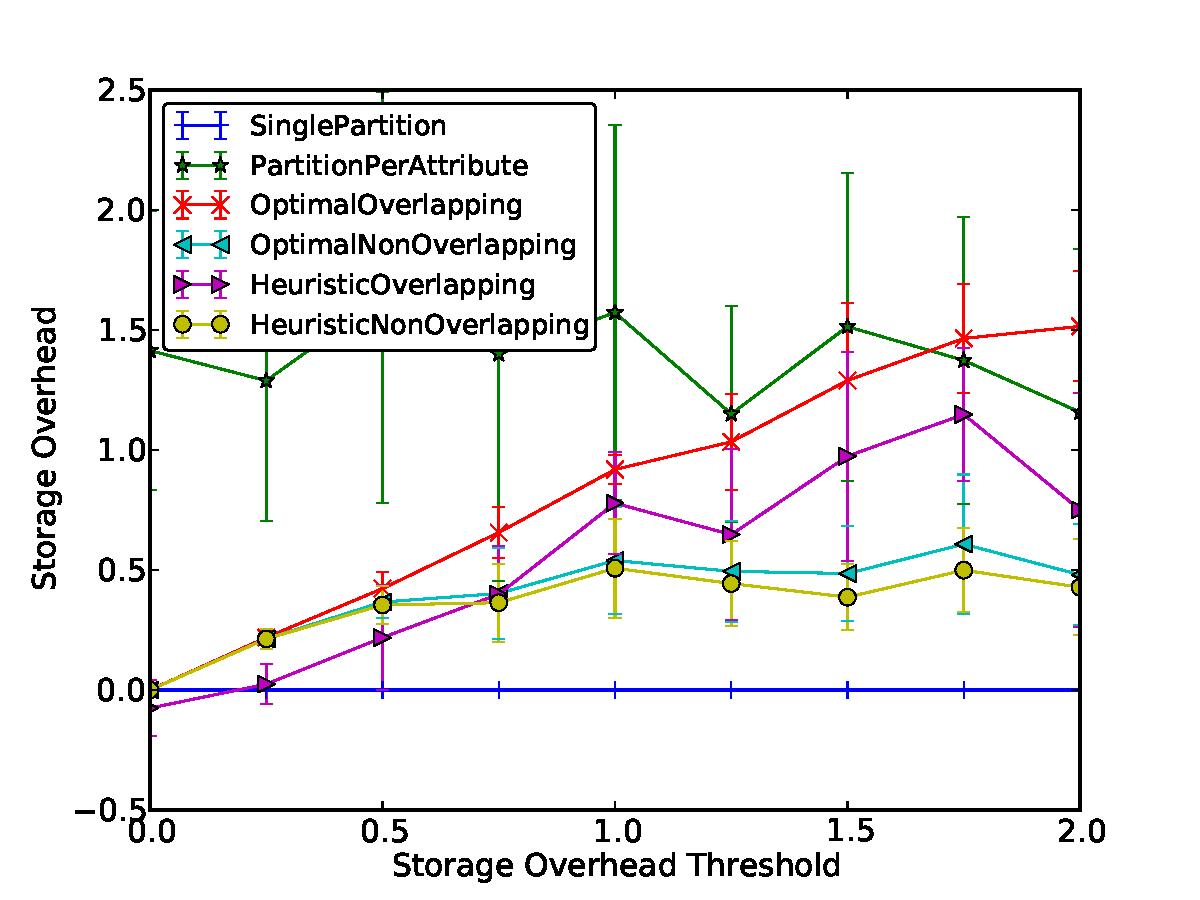
\includegraphics[width=0.33\textwidth]{figures/StorageOverheadVsStorageOverheadThreshold.pdf}\\
 (a)Num Attributes & (b) NumQueryKind &
 (c) StorageOverheadThreshold \\
 \end{tabular}}
\vspace*{1mm}
 \caption{Running time, QueryIO, and StorageOverhead.}
 \label{fig:results}
 \end{figure*}


\section{Related Work}

\begin{alltt}\scriptsize
Gedik et al.~\cite{gedik14}
H2O \cite{alagiannis14}
HYRISE~\cite{grund10}
Bornea et al.~\cite{bornea13}
\end{alltt}


\bibliographystyle{abbrv}
\bibliography{paper}  
\end{document}
